% !TeX root = RJwrapper.tex
\title{\pkg{pCODE}: Estimating Parameters of ODE Models}
\author{by Haixu Wang and Jiguo Cao}

\maketitle

\abstract{
  The ordinary differential equation (ODE) models are prominent to characterize the mechanism of dynamical systems with various applications in biology, engineering, and many other areas. While the form of ODE models is often proposed based on the understanding or assumption of the dynamical systems, the values of ODE model parameters are often unknown. Hence, it is of great interest to estimate the ODE parameters once the observations of dynamic systems become available. The parameter cascade method initially proposed by \cite{parcascade} is shown to provide an accurate estimation of ODE parameters from the noisy observations at a low computational cost. This method is further promoted with the implementation in the R package \pkg{CollocInfer} by \cite{CollocInfer}. However, one bottleneck in using \pkg{CollocInfer} to implement the parameter cascade method is the tedious derivations and coding of the Jacobian and Hessian matrices required by the objective functions for doing estimation. We develop an R package \pkg{pCODE} to implement the parameter cascade method, which has the advantage that the users are not required to provide any Jacobian or Hessian matrices. Functions in the \pkg{pCODE} package accommodate users for estimating ODE parameters along with their variances and tuning the smoothing parameters. The package is demonstrated and assessed with four simulation examples with various settings. We show that \pkg{pCODE} offers a derivative-free procedure to estimate any ODE models where its functions are easy to understand and apply. Furthermore, the package has an online Shiny app at \url{https://pcode.shinyapps.io/pcode/}.
}

\section{Introduction}\label{sec:introduction}
The evolution of a dynamic system in time can be represented by ordinary differential equations (ODE) models consisting of a set of state variables and their derivatives. For example, the state variables can be the population of multiple species in an ecological system, the velocities, and locations of particles in a physics system, the concentration of chemicals in a reactor, or the energy of objects in a heating process. Usually, an ODE model is defined as a set of differential equations in the following form
\begin{equation}
\dot{\bm{x}}(t) = \bm{f}(\bm{x},\bm{u},t|\bm{\theta}),
\label{eq:generalode}
\end{equation}
where $\bm{x}(t)$ denotes the fully or partially observed states of the system at time $t$. The ODE model links the first derivative, the temporal change, of the states with $\bm{x}$ itself and other influential components $\bm{u}$ through some function $\bm{f}$ defined by the parameter vector $\bm{\theta}$. \par


%Literature review on solving an ODE system or estimating parameters 
Conventionally, parameter estimation of an ODE model combines numerically solving the system and updating the ODE parameters given the solution. The updating step complies with the nonlinear regression framework as suggested in \cite{nonlinearestBARD} and \cite{nonlinearparameterestimation}. That is, the optimal $\bm{\theta}$ minimizes the sum of squared errors between the observations and the solutions of ODE models. It is not very typical for an ODE model to have analytical solutions unless the dynamic system is simple and linear. In more realistic situations where analytical solutions are not available, the ODE solutions must be numerically obtained prior to any estimations of the ODE parameters. The initial condition, which are values of state variables at the initial time, dictates the unique solution obtained by the numeric solver. However, the initial condition is often unavailable in real practices and must be estimated before obtaining the ODE solutions. If the initial conditions are unknown, then they are augmented to the parameter vector and estimated simultaneously with the ODE parameters. As a result, the complexity of optimization dramatically increases due to the fact that the solution is sensitive to ODE parameters and initial conditions. Also, the augmentation increases the dimension and complexity of the optimization surface hence hindering the convergence of optimization algorithms.

Being an improvement in the stability of estimation, the multiple shooting methods, presented in \cite{BOCKmultiple}, \cite{peifermultiple}, and \cite{nonlineardynamic}, expands the dimension of optimization surface by introducing additional initial conditions. The extra initial conditions are a result of partitioning the original time interval into multiple subintervals, and numeric solutions are obtained within each subinterval. Ideally, the introduction of these initial conditions will facilitate the optimization process for $\bm{\theta}$ to avoid local minima in the optimization surface and provide a faster convergence rate. Additionally, \cite{Huang_bayesian} and \cite{Gelman_bayesian} present Bayesian frameworks of estimating ODE parameters with a hierarchical model. 

The aforementioned strategies depend on the numeric solutions of ODE models and can be burdened with significant computational challenges given complex dynamic systems. That is, the system has to be numerically solved given each update or candidate of ODE parameters. To overcome these challenges, \cite{Varah} proposes a two-step procedure to use nonparametric techniques for interpolating the time derivatives of state variables. Subsequently, the parameters are estimated through a nonlinear regression framework by treating the time derivatives as the response. This methodology is further developed in  \cite{wu_localestimation}, \cite{ramsayFDA} , and \cite{brunel2008}. Replacing numeric solutions with nonparametric estimations drastically reduces the computational cost, but estimation errors are introduced in the process of interpolating the time derivatives. The errors are due to the fact that there are no direct observations of the derivatives. Furthermore, \cite{varyingODE} shows that the estimation errors of derivatives will lead to bias in the estimation of ODE parameters. 

As contrary to the two-step procedure, \cite{parcascade} presents a new approximation strategy, called the parameter cascade method, in the family of collocation methods. The parameter cascade method integrates data smoothing and estimation of ODE parameters into a single estimation scheme. The parameter cascades method provides a much more efficient way of approximating the ODE solution without numerically solving the system. Additionally, it ensures that the ODE parameters are more accurately estimated than the two-step approach \citep{varyingODE}. Various well-known ODE models are examined in \cite{parcascade}. \cite{qi2010} has discussed the asymptotic properties of the parameter cascades estimates for both ODE parameters and basis coefficients. The methodology has also been validated with many applications. \cite{selectionofODE} investigates the model selection problem in ODE models based on parameters estimated from the cascading procedure. When the system is measured with replications, mixed effects need to be incorporated into the model. This mixed-effect ODE model is explored in \cite{ODEmixedeffect}. 

The cascading estimation strategy is further promoted as in the R package \pkg{CollocInfer} by \cite{CollocInfer}. \pkg{CollocInfer} offers a variety of functions regarding the estimation of ODE models. It has included the implementation of the parameter cascade method, the tuning criterion of smoothing parameter, and the sample variance of parameter estimates through the Newey-West method in \cite{neweywest}. However, one bottleneck of using \pkg{CollocInfer} is the requirement of manually providing all the partial derivatives for constructing the Jacobian and Hessian matrices in the optimization process. For complex ODE models, the calculation and coding of those derivatives can be tedious and easy to make mistakes. As an improvement to the \pkg{CollocInfer} package, we propose a new package, named \pkg{pCODE}, which offers more user-friendly functions for estimating ODE models without specifying any derivatives. That is, an analytic Jacobian and Hessian matrix is required for the optimization routine in \pkg{CollocInfer}, whereas \pkg{pCODE} automatically calculates the numeric approximations to both matrices. Furthermore, \pkg{pCODE} also adds a bootstrap variance estimator besides the variance estimator obtained by the Delta method in \cite{parcascade} and \pkg{CollocInfer}. \pkg{pCODE} uses the k-fold cross-validation for finding the optimal smoothing parameter while \pkg{CollocInfer} selects the smoothing parameters based on the forward prediction errors. We have also developed an online Shiny app at \url{https://pcode.shinyapps.io/pcode/}.

The remainder of this paper is organized as follows. Next section will introduce the parameter cascade methodology for simultaneous estimation of both ODE solutions $\bm{x}(t)$ and parameters $\bm{\theta}$. The third section explains the core functions of the package \pkg{pCODE} along with their usages and syntaxes. Subsequently, The fourth section illustrates the application of \pkg{pCODE} on several datasets with simulations for assessing the performance. At last, The fifth section gives a conclusion of the paper. 


\section{The parameter cascade method} \label{seq:method}
An ODE model is build upon a set of differential equations $\dot{x}_{i}(t) = f_{i}(\bm{x},t|\bm{\theta})$ for $i = 1,..., I,$ corresponding to the index of state variables. Each differential equation represents how the time derivative of one state variable depends on $\bm{x} = (x_{1},..., x_{I})$. Furthermore, $f_{i}(\bm{x},t|\bm{\theta})$'s are assumed to be parametrized by a vector of parameters $\bm{\theta}$. Let $y_{ij} = x_{i}(t_{ij}) +  e_{ij}$ be the $j$-th noisy observation of $i$-th state variable at time $t_{ij}$, where $e_{ij}$ is the measurement error or noise, $j = 1, ..., n_{i}$. We assume the vector of random errors $\bm{e}_{i} = (e_{i1},...,e_{in_{i}})$ has a distribution function $g(\bm{e}_{i})$ with the distribution parameter $\bm{\sigma}_{i}$. Our goal is to estimate $\bm{\theta}$ from the noisy observations from the system. 

The lower stream estimation of the parameter cascade method is to provide smooth interpolations of the observations. As suggested in \cite{parcascade}, the data interpolation part is done by the smoothing splines. The goal of smoothing is to diminish the random errors in the observations of all dimensions, hence the underlying solutions $x_{i}(t)$'s can be recovered from the noisy observations. That is, each $x_{i}(t)$ is expressed as a linear combination of B-spline basis functions
\begin{equation*}
     x_{i}(t) = \sum_{i}^{K_{i}} c_{ik} \phi_{ik}(t) = \bm{c}^{\prime}_{i}\bm{\phi}_{i}(t),
\end{equation*}
where $K_{i}$ is the number of basis functions, and $\bm{\phi}_{i}(t)$ is the vector of basis functions evaluated at a time point $t$. Data smoothing is then equivalent to the estimation of these basis coefficients $\bm{c}_{i}$'s. 

%Normally, the optimal $K_{i}$ is obtained through a tuning process. A larger $K_{i}$ leads to overfitting and wiggly estimates of the ODE solutions, and insufficient number of basis functions cannot provide a satisfactory interpolation to capture the variation in both $x_{i}(t)$ and its derivative. Selecting optimal $K_{i}$'s for all dimensions can be computationally tedious and indecisive for a given search grid. 
%For that matter, the penalization approach remedies the situation by imposing a smoothness constraint within the optimization for obtaining basis coefficients. Hence, a saturated number of basis functions, i.e., putting one knot at each time with observations, can be used without the consequence of overfitting the observations and left to be a subjective matter. Consequently, the numeric solutions $x_{i}(t)$ can be fully reconstructed based on the estimation basis coefficients $\bm{c}_{i}$. The initial condition $x_{i}(t_{i1})$ is also immediately estimated as $\hat{x}_{i}(t_{i1})$. 

To comply the lower level estimation, a simple objective function $J(\bm{c})$, following the smoothing spline routine, is considered for obtaining basis coefficients $\bm{c} = (\bm{c}^{\prime}_1,\ldots,\bm{c}^{\prime}_I)^{\prime}$. That is, the negative log-likelihood function is chosen for non-normal errors, whereas the least square criterion is naturally suitable for i.i.d. normal errors $e_{ij} \sim \text{N}(0,\sigma_{i})$. The summation $J(\bm{c}|\bm{\sigma}) = \sum_{i} J(\bm{c}_{i}|\bm{\sigma}_{i})$ of individual fitting criterion over $i$ defines a composite objective function for all $I$ dimensions. The data interpolation will use a saturated number of basis functions which requires a penalty term in the objective function to prevent overfitting problems. \cite{ramsayFDA} suggests to use a linear differential operator for introducing a smoothness penalty in the objective functions. Subsequently, \cite{Poyton2006} utilizes the smoothness penalty in estimating parameters and solutions of ODE models. Following the same technique, the smoothness penalty is defined based on the discrepancy between the time derivatives and the ODE model, i.e., 
 \begin{equation}
       \int (\dot{x}_{i}(t) - f_{i}(\bm{x},t|\bm{\theta}))^{2}dt,
 \end{equation}
 for each state variable $x_{i}$. Multiplying the penalty with a smoothing parameter $\lambda_{i}$ and combining the penalties over all dimensions, the complete objective function is defined to be 
 \begin{equation}
  J(\bm{c}|\bm{\theta}) = \sum_{i=1}^{I} \big[ - \ln g(\bm{e}_{i}) + \lambda_{i}\int (\dot{x}_{i}(t) - f(\bm{x},t|\bm{\theta}))^{2}dt\big].
  \label{eq:innerobj}
 \end{equation}
 For each given set of ODE parameters $\bm{\theta}$, the basis coefficients $\bm{c}$ is estimated by minimizing $J(\bm{c}|\bm{\theta})$. Hence, the estimate for the basis coefficients $\bm{c}$ become an implicit function of the ODE parameters $\bm{\theta}$ as $\bm{c}(\bm{\theta})$. The objective function (\ref{eq:innerobj}), referred to as the inner objective function, needs to be optimized for estimating $\bm{c}$ whenever $\bm{\theta}$ is updated. 

 %Terminologies of parameters
To clearly distinguish two sets of parameters $\bm{c}$ and $\bm{\theta}$, $\bm{c}$ will be referred to as the nuisance parameters since they are not essential for estimating the ODE model rather interpolate the observations. On the other hand, $\bm{\theta}$ is responsible for defining the structure of the ODE model and will be denoted as structural parameters. Often, $\bm{\theta}$ will be the primary concern given any ODE models. 

The upper stream estimation of the parameter cascade method focuses on the structural parameter $\bm{\theta}$. To comply this estimation, the objective function $H(\bm{\theta})$, referred to as the outer objective function, is optimized with respect only to the structural parameters $\bm{\theta}$. It is usually defined to be the negative log-likelihood function or the sum of squared errors given the distributions of random errors, that is,
\begin{equation}
H(\bm{\theta}) = -\sum_{i=1}^{I}\text{ln }g(\widehat{\bm{e}}_{i}|\bm{\theta}),
\label{eq:outterobj}
\end{equation}
where
\begin{equation*}
\widehat{\bm{e}}_{i} = \bm{y}_{i} - \hat{x}_i(\bm{t}_{i}|\bm{\theta}).
\end{equation*}
Here $\hat{x}_i(\bm{t}_{i}|\bm{\theta}) = \hat{\bm{c}}^{\prime}_{i}(\bm{\theta})\bm{\phi}_{i}(\bm{t}_{i})$, where $\hat{\bm{c}}^{\prime}_{i}(\bm{\theta})$ is the optimizer of $J(\bm{c}|\bm{\theta})$ given current $\bm{\theta}$. 

The parameter cascade method nests the estimation of basis coefficients in that of the structural parameters, where both estimations depend on the choice of smoothing parameters $\bm{\lambda}$. As a result, the interpolation of data points is not separated from estimating ODE parameters. The stream of dependencies defined a parameter cascade which offers great accuracy and efficiency in estimating ODE models. To take full advantage of the parameter cascade method, the \pkg{pCODE} package provides several R functions that are able to apply the aforementioned methodology for estimating ODE models. 



\section{Main functions in the pCODE package } \label{seq:functions}
\subsection[pcode]{Parameter estimation: \code{pcode}}
The main function to perform the parameter cascade method is \code{pcode} in the package. This is a generic wrapper function for handling several scenarios given different objective functions, normal or non-normal errors, and missing state variables. 


First, we focus on the situation when we have the normal random errors for all dimensions where $e_{ij}\sim\text{N}(0,\sigma^{2}_{i})$. In fact, both the inner optimization function (\ref{eq:innerobj}) and the outer optimization function (\ref{eq:outterobj}) are calculated based on a vector of residuals. The first part of (\ref{eq:innerobj}) is easily recognized as the residuals from fitting the observation with basic functions. If the second part, the integral, is approximated by the composite Simpson's rule, then the approximation can be written in a quadratic form based on a vector of residual-like quantities. Stringing the aforementioned two vectors into one, and the concatenation of these vectors from all dimensions will produce a single vector of residuals. Hence, the optimization of the inner objective function adheres to the non-linear least square (NLS) framework. As a result, we can use the popular Levenberg-Marquart (LM) algorithm to obtain an estimate $\hat{\bm{c}}^{\prime}_{i}(\bm{\theta})$. Our package \code{pcode} employs the function \code{lsqnonlin} from the package \pkg{PRACMA} \citep{pracma} for applying the LM algorithm. 

The optimization of the outer objective function appears to be exactly an NLS problem. However, the parameter cascade strategy appends an extra layer of optimization to each update of the outer estimation, which characterizes a nested optimization problem. It is applicable to apply the Levenberg-Marquart algorithm again to the outer objective, however, the computational effort is much greater than that of inner optimization. The reason is that a Jacobian matrix needs to be calculated for each iteration of the update on the structural parameters, and each entry of the Jacobian for the outer objective involves a complete optimization of the inner one. This occurs to be the major delay in computation time. 

Most commonly, the random errors $e_{ij}$'s are i.i.d from the normal distribution. However, some dynamic systems may produce non-normal errors which make the NLS approach not applicable. One solution is to perform a transformation on the observations and state variables, which forces the errors of transformed variables to have a normal distribution. As an alternative, \code{pcode} allows one to input a likelihood (or log-likelihood) function as a fitting criterion for both inner and outer objectives. In such a case, \code{optim} will be used for both levels of objective functions. 

The following demonstrates the syntax of \code{pcode} with its argument list:
\begin{example*}
pcode(
  data, time, ode.model, par.names, state.names, likelihood.fun,
  par.initial, basis.list, lambda, controls
)
\end{example*}
where \code{data}, a matrix, contains the observations of state variables as columns. The names of state variables are stored in \code{state.names} as a vector. \code{time} includes the observation time points in a vector. The ODE model to be estimated is provided to \code{pcode} as \code{ode.model} and defined in a similar way as that in package \pkg{deSolve} \citep{deSolve}:

\begin{example*}
ode.model <- function(t, state, parameters) \{
  with(as.list(c(state, parameters)), \{
    dV <- c * (V - (V^3) / 3 + R)
    dR <- -(1 / c) * (V - a + b * R)
    return(list(c(dV, dR)))
  \})
\}
\end{example*}


For this example, the state names are passed to the function \code{PCODE} as a vector \code{c('V','R')}, and the structural parameter names \code{c('a','b','c')} are given to \code{par.names} argument of the function. Optimization for the structural parameters requires a initial value input as \code{par.initial}, and there is no need for an input of \code{likelihood.fun} when the error distributions are Normal. \code{basis.list} contains the list of basis objects defined by the package \pkg{fda}, and the default \code{basis} has 9 interior knots with B-spline basis functions of order of 4. \code{lambda} corresponds to the penalty parameter $\bm{\lambda}$ which controls the fitness of estimated state variables to the differential equations. A scalar input of \code{lambda} means that all dimensions will subject to the same penalty, or a vector input differentiates the penalty calculated for each dimension. \code{controls} contains addition parameters to adjust optimizations for both inner and outer objective functions and obtain initial value for basis coefficients $\bm{c}$. Two scenarios are discussed depending on the different distribution of errors. All the mentioned scenarios will be demonstrated in the fourth section with examples.

\subsubsection[bootsvar]{The bootstrap variance estimator: \code{bootsvar}}
All the functions of this package are derivative-free, hence the variance of structural parameters is numerically approximated. The first option is to use the bootstrap variance estimator. Given the estimation of both parameters $\bm{\theta}$ and $\bm{c}$, we are able to solve the ODE directly with estimated initial value $\hat{\bm{x}}(t_{0})$. Hence, we can simulate bootstrap samples of the ODE model based on the estimated distributions of errors $\bm{e}_{i}$ for all $I$ dimensions. The detailed algorithm for obtaining a bootstrap variance estimate of $\bm{\theta}$ is as follows

\begin{algorithm}[H]
  \caption{Bootstrap variance estimator
    \label{alg:bootsvar}}
  \begin{algorithmic}
    \Require{}\\
    \begin{itemize}
      \item  $\bm{\theta}_{0}$: initial value for structural parameters
      \item  $B$: the number of bootstrap samples
      \item  $\bm{y}$: observations
      \end{itemize}

    \Statex
    \Function{Bootsvar}{$\bm{\theta}_{0}, B, \bm{y}...$}
      \Let{$\bm{\theta}_{\star},\bm{c}_{\star}$}{results from \code{pcode($\bm{\theta}_{0},\bm{y}...$)}}  \Comment{Estimation from the original data}
      \Let{$\sigma_{i}^{2}$\hspace*{1.4em}}{var($\bm{y}_{i} - \bm{x}_i$)} \Comment{Estimate the variance of observation errors}
      \Let{$\bm{x}_{\star}$\hspace*{1.4em}}{Solution to the ODE given $\bm{\theta}_{\star}$ and $\bm{x}_{\star}(t_{0})$}
      \For{$b \gets 1 \textrm{ to } B$}
          
            \hspace*{1em}Obtain $\bm{z}_{i}^{(b)}$ = $\bm{x}_{i,\star}+\bm{\epsilon}_{i}^{(b)}$.      \Comment{$\bm{\epsilon}_{i}^{(b)} \sim N(0,\sigma_{i}^{2})$}

            \Let{($\bm{\theta}_{\star}^{(b)},\bm{c}_{\star}^{(b)}$)}{results from \code{pcode($\bm{\theta}_{\star},\bm{z}_{i}^{(b)}...$)}}
          

      \EndFor
      \State \Return{$Var(\bm{\theta}_{\star}^{(b)}),Var(\bm{c}_{\star}^{(b)})$}
    \EndFunction
  \end{algorithmic}
\end{algorithm}
The syntax of \code{bootsvar} is illustrated as the following

\begin{example*}
bootsvar(
  data, time, ode.model, par.names, state.names, par.initial,
  lambda, basis.list, bootsrep, controls
)
\end{example*}

Most of the arguments are the same as the function \code{pcode} with only one addition of argument \code{bootsrep} which indicates the number of bootstrap samples to be taken for obtaining the variance estimator. 



\subsubsection[deltavar]{The Delta variance estimator: \code{deltavar}}
As an alternative to the bootstrap variance estimator, the package \pkg{PCODE} also offers another numeric estimator for the variance of structural parameters. \cite{parcascade} has developed the approximation to $Var(\bm{\hat{\theta}}(\bm{y}))$ via the delta-method. The resulting approximation is of the form 
\begin{equation*}
Var(\hat{\bm{\theta}}(\bm{y})) \approx \bigg[ \frac{d\bm{\hat{\theta}}}{d\bm{y}} \bigg] \bm{\Sigma}  \bigg[ \frac{d\bm{\hat{\theta}}}{d\bm{y}} \bigg]^{\prime}
\end{equation*} 
where $\frac{d\bm{\hat{\theta}}}{d\bm{y}}$ is obtained as 
\begin{equation}
  \label{eq:dtheta_dy}
 \frac{d\bm{\hat{\theta}}}{d\bm{y}} = - \bigg[\frac{\partial^{2}H}{\partial\bm{\theta}^2}\bigg\vert_{\bm{\hat{\theta}}(\bm{y})} \bigg]^{-1} \bigg[  \frac{\partial^{2}H}{\partial\bm{\theta}\partial\bm{y}}\bigg\vert_{\bm{\hat{\theta}}(\bm{y})} \bigg]
\end{equation}
and $\bm{\Sigma}$ is a $N \times N$ variance-covariance matrix for observations put into a vector. $N$ is the total number of observation summing over all dimensions of $\bm{y}$
. Then the estimation of variance relies on the computation of (\ref{eq:dtheta_dy}). The partial derivatives are approximated by the finite difference method, i.e., 
\begin{equation*}
\bigg[\frac{\partial^{2}H}{\partial\bm{\theta}_{u}^2}\bigg\vert_{\bm{\hat{\theta}}(\bm{y})} \bigg] \approx \frac{H(\hat{\bm{\theta}}_{u+}(\bm{y})|\bm{\lambda}) - 2H(\hat{\bm{\theta}}(\bm{y})|\bm{\lambda}) + H(\hat{\bm{\theta}}_{u-}(\bm{y})|\bm{\lambda})}{\Delta^{2}},
\end{equation*}
where $\hat{\bm{\theta}}_{u+}(\bm{y})$ and $\hat{\bm{\theta}}_{u-}(\bm{y})$ indicate the addition and subtraction of stepsize $\Delta$ to the u-th structural parameter estimate $\hat{\bm{\theta}}(\bm{y})$. The mixed partial derivatives are approximated as the following
\begin{equation*}
\bigg[\frac{\partial^{2}H}{\partial\bm{\theta}_{u}\partial\bm{\theta}_{v}}\bigg\vert_{\bm{\hat{\theta}}(\bm{y})} \bigg] \approx \frac{H(\hat{\bm{\theta}}_{u+,v+}(\bm{y})) - H(\hat{\bm{\theta}}_{u-,v+}(\bm{y})) - H(\hat{\bm{\theta}}_{u+,v-}(\bm{y})) +H(\hat{\bm{\theta}}_{u-,v-}(\bm{y}))}{4\Delta^{2}}.
\end{equation*}
Given any fixed argument $\bm{\theta}$ for the outer objective function $H(\bm{\theta},\bm{\sigma}|\bm{\lambda})$, its evaluation involves the profiled estimation of $\bm{c}(\bm{\theta},\bm{\sigma};|\bm{\lambda})$ and returns solely the likelihood or the sum of squared errors. Hence, individual evaluations of $H(\bm{\theta},\bm{\sigma}|\bm{\lambda})$ used in numeric approximation is obtained in the following steps:
\begin{itemize}
  \item Step 1: Optimize $J(\bm{c}|\bm{\theta},\bm{\lambda})$ given $\bm{\theta}$.
  \item Step 2: Obtain $\hat{\bm{x}}(\bm{t})$ based on the estimated $\hat{\bm{c}}$.
  \item Step 3: Return $\sum_{i \in I} ||\bm{y}_{i} - \hat{x}_{i}(\bm{t}_i)||^{2}$ or $-\sum_{i \in I}g(\bm{y}_{i} - \hat{x}_{i}(\bm{t}_i)|\bm{\theta},\bm{\lambda})$.
  \end{itemize}
Approximation to the second term $\frac{\partial^{2}H}{\partial\bm{\theta}\partial\bm{y}}\bigg\vert_{\bm{\hat{\theta}}(\bm{y})}$ utilizes the finite difference method as well. After evaluating $H(\bm{\theta},\bm{\sigma}|\bm{\lambda})$ given $\bm{\theta}$, the mixed partial derivative is calculated by moving the particular observation up or down by some stepsize $\Delta_{y}$. That is,
\begin{equation*}
\bigg[\frac{\partial^{2}H}{\partial\bm{\theta}_{u}\partial y_{v}}\bigg\vert_{\bm{\hat{\theta}}(\bm{y})} \bigg] \approx \frac{H(\hat{\bm{\theta}}_{u+},\bm{y}_{v+}) - H(\hat{\bm{\theta}}_{u+},\bm{y}_{v-}) - H(\hat{\bm{\theta}}_{u-},\bm{y}_{v+}) +H(\hat{\bm{\theta}}_{u-},\bm{y}_{v-})}{4\Delta\Delta_{y}},
\end{equation*}
where $\bm{y}_{v+}$ and $\bm{y}_{v-}$ represent moving up and down v-th observation by stepsize $\Delta_{y}$ in the last step of evaluating $H(\bm{\theta},\bm{\sigma}|\bm{\lambda})$.  
The syntax of \code{numericvar} is based on that of \code{pcode}

\begin{example*}
numericvar(
  data, time, ode.model, par.names, state.names,
  par.initial, lambda, basis.list, stepsize, y_stepsize, controls
)
\end{example*}

with addition of \code{stepsize} and \code{y\_stepsize}. \code{stepsize} can be specified by a single number for which finite difference method will use it for all parameters or a vector where derivative of each parameter is estimated based on its own stepsize. \code{y\_stepsize} allows an input of a vector where each element indicates the stepsize for each dimension of the ODE model. 
\section{Illustrations} \label{sec:illustrations}
\subsection{A simple ODE model} \label{ssec:simpleode}
A simple illustration uses an one-dimensional ODE model
\begin{equation}
\dot{X} = \theta X (1-\frac{X}{10}).
\label{eq:simpleode}
\end{equation}
The following code defines the aforementioned model that will be provided for \code{pcode} for estimating parameters:
\begin{example*}
model <- function(t, state, parameters) \{
  with(as.list(c(state, parameters)), \{
    dX <- theta * X * (1 - X / 10)
    return(list(dX))
  \})
\}
\end{example*}
Given an observation period of $[0,100]$, random noise errors are added to the ODE solution with a Normal distribution $\text{N}(0,0.5^{2})$. Observations of the system are generated as follows:
\begin{example*}
times  <- seq(0, 100, length.out = 101)
mod    <- ode(y = state, times = times, func = ode.model, parms = model.par)
nobs   <- length(times)
scale  <- 0.5
noise  <- scale * rnorm(n = nobs, mean = 0, sd = 1)
observ <- mod[, 2] + noise
\end{example*}

Subsequently, we can visualize the observations along the true solution of this simple ODE model in Figure~\ref{fig:simpledata}.
\begin{figure}[H]
\centering
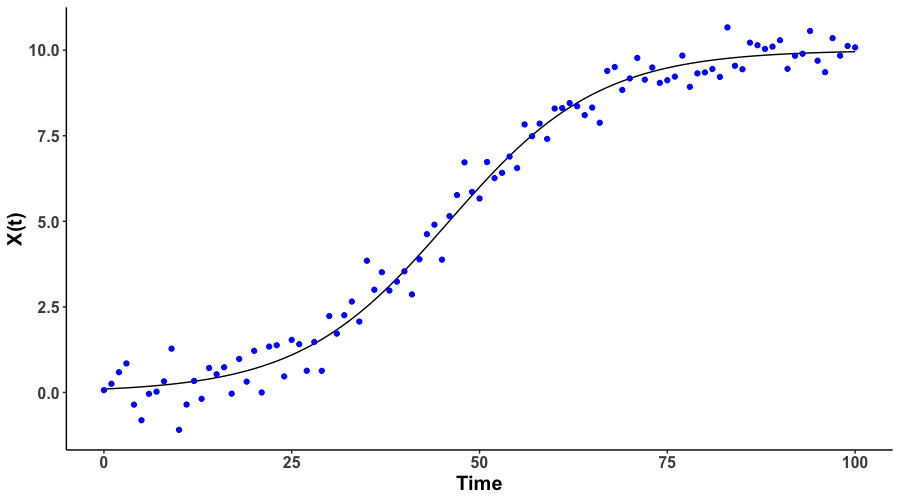
\includegraphics[width=\textwidth]{simple_ode_observation.png}
\caption{\label{fig:simpledata} This plot demonstrates the solution of an ODE system. The black solid line represents the true ODE solution given a known initial value. The estimation of the solution and parameters of the ODE system usually depends on some noisy observations of the system. The noisy observations, the blue points, are used for estimation.}
\end{figure}
First, a basis object needs to be defined by \code{create.bspline.basis} from \pkg{fda} package
\begin{example*}
knots  <- seq(0, 100, length.out = 21)
norder <- 4
nbasis <- length(knots) + norder - 2
basis  <- create.bspline.basis(c(0, 100), nbasis, norder, breaks = knots)
\end{example*}
A B-spline basis is created given 21 konts including both interior and boundary knots acorss observation interval $(0,100)$. The order of basis functions is 4, so there is a total of 23 basis functions. To perform the parameter cascade method for estimating both structural and nuisance parameters, one can use \code{pcode} in the following way
\begin{example*}
pcode.result <- pcode(
  data = observ, time = times, ode.model = model,
  par.initial = 0.3, par.names = "theta", state.names = "X",
  basis.list = basis, lambda = 1e2
)
pcode.result["structural.par"]
theta
0.09995229
\end{example*}
To validate the methodology of this function, data simulation and parameter estimation are repeated for 100 times.
\begin{figure}[H]
    \centering
    \begin{subfigure}[t]{0.5\textwidth}
        \centering
        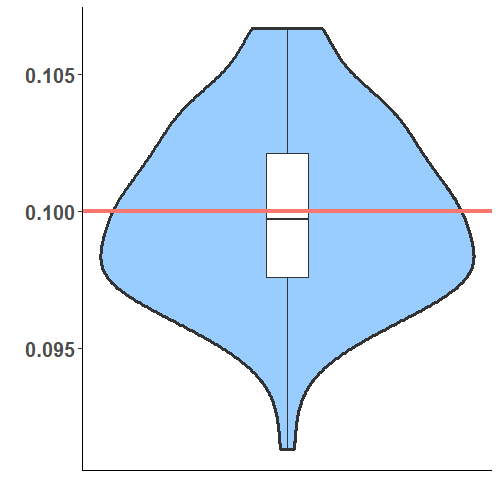
\includegraphics[width=\textwidth]{simple_ode_estpar.png}
        \caption{The violin and boxplot of the estimated $\theta$ over 100 replications.}
    \end{subfigure}%
    ~ 
    \begin{subfigure}[t]{0.5\textwidth}
        \centering
        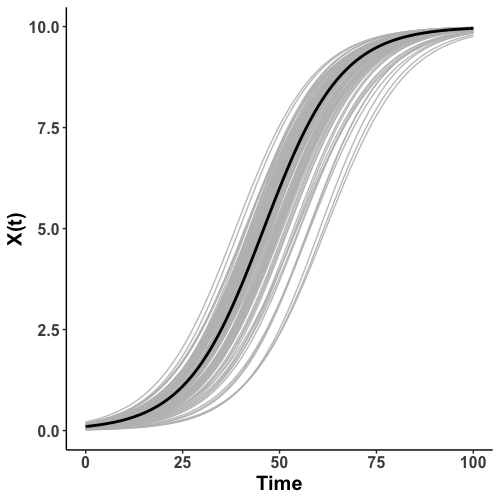
\includegraphics[width=\textwidth]{simple_ode_solve.png}
        \caption{Solution of the ODE model with $\hat{\theta}$ and $\hat{X}(0)$.}
    \end{subfigure}
    \caption{\label{fig:simpleresult} The violin plot demonstrates the reliability of the estimation procedure. It summarizes the estimates of parameters over 100 replications. Each replication generates a entirely new set of noisy observations and gives a parameter estimate of the simple ODE model (\ref{eq:simpleode}). The true parameter is indicated by the redline as $\theta = 0.1$. The right plot shows the estimation of the solution from the simple ODE model over 100 replications. Each grey line is obtained from solving the ODE system after obtaining the parameter estimate from one replication. The black curve is the ODE solution with the true value of $\theta$. }
\end{figure}
Given that $\theta = 0.1$ is used for generating data, the parameter cascade method performs impressively well. The violin plot in Figure~\ref{fig:simpleresult} shows that the distribution of estimates of $\theta$ covers 0.1 (indicated by the red horizontal line) and does not fall far away from the true value. Also, the state variable \code{X} (the bold black curve of the plot on the right) is well predicted by solving the ODE model with estimated initial value $\hat{x}(0)$ and structural parameters $\hat{\theta}$.


The true variance for data generating parameter $\theta$ is $1.003 \times 10^{-5}$. We can compare the performance of two functions \code{bootsvar} and \code{deltavar} for estimating $\text{var}(\theta)$. 
\begin{example*}
bootsvar(
  data = observation, time = times, ode.model = ode.model,
  par.initial = 0.3, par.names = "theta", state.names = "X",
  basis.list = basis, lambda = 1e2, bootsrep = 20
)
theta
1.042763e-05

deltavar(
  data = observation, time = times, ode.model = ode.model,
  par.initial = 0.3, par.names = "theta", state.names = "X",
  basis.list = basis, lambda = 1e2,
  stepsize = 1e-5, y_stepsize = 1e-5
)
theta
9.923318e-06
\end{example*}
Both variance estimator give excellent estimates of the true variance of structural parameter. Subsequently, the consistency and reliability of those estimator can be inspected by simulation. In 100 simulation replicates, the results of two variance estimators are summarized in Figure \ref{fig:sipmleode_varestimate}.
\begin{figure}[H]
  \centering
  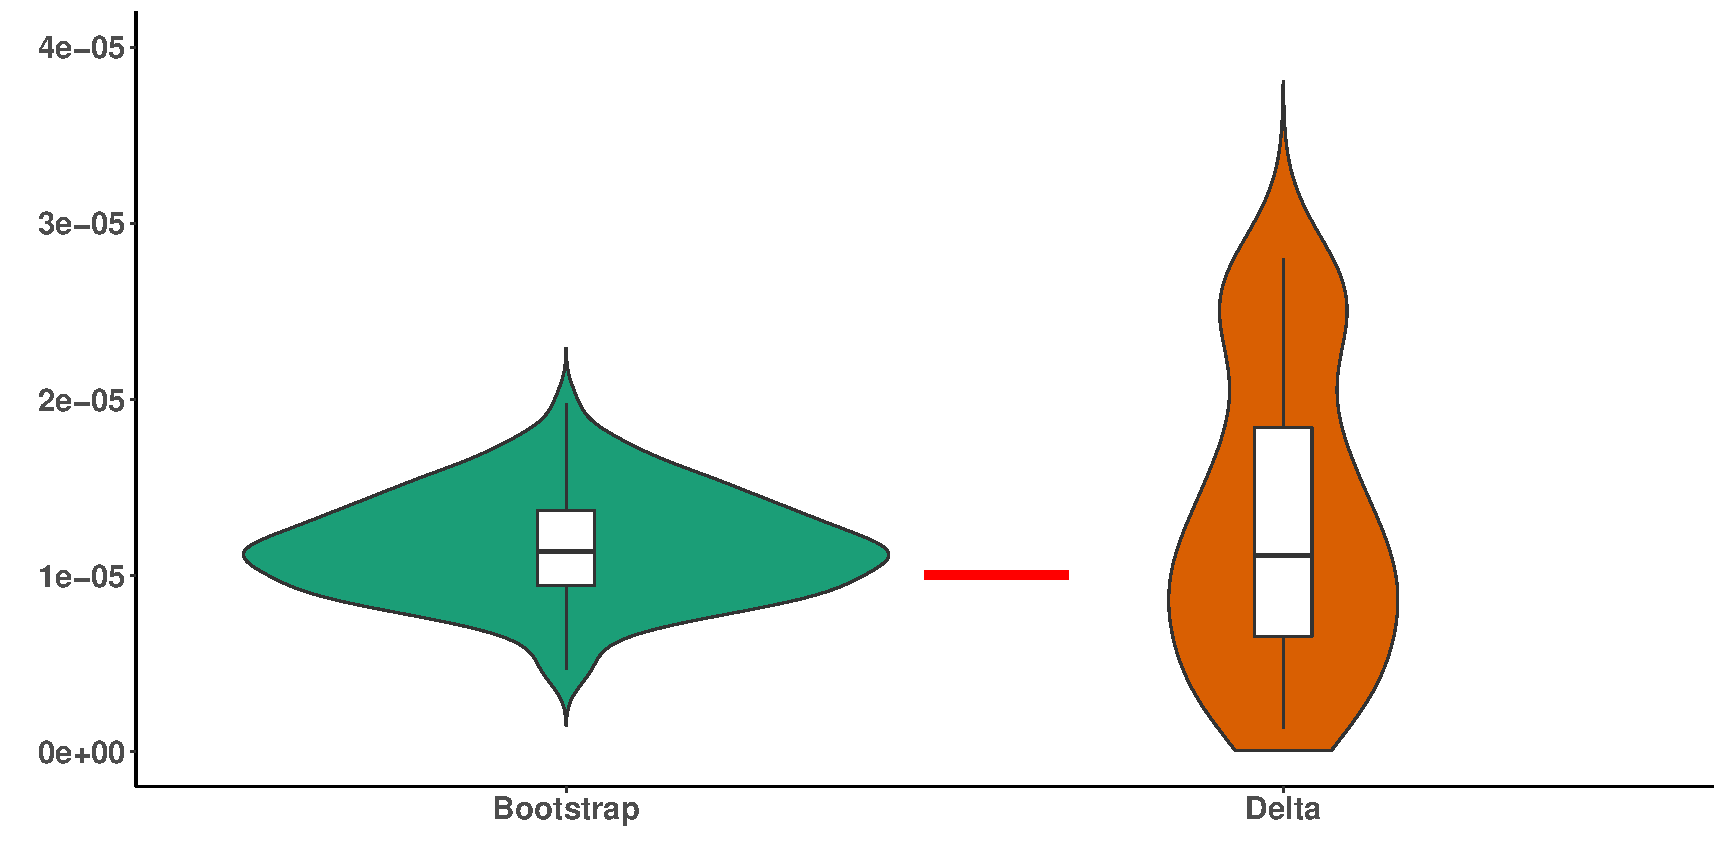
\includegraphics[width=\textwidth]{comparevar.pdf}
  \caption{\label{fig:sipmleode_varestimate} This plot demonstrates the estimation of variance of parameters over 100 replications. Two violin plots are results from two methods, the bootstrap and Delta method, introduced in the article. The red line segment indicates the true variance. Green plot includes the estimates from the bootstrap method, whereas the origin plot includes those from the Delta method.}
\end{figure}

The bootstrap variance estimator has a smaller variation but at the cost of higher computational effort in comparison with the Delta variance estimator. On the other hand, the Delta variance estimator is faster but sensitive to the choice of the step size in estimating all the derivatives and the subsequent $\text{var}(\theta)$.

\subsection{The FitzHugh-Nagumo ODE model}
The FitzHugh-Nagumo ODE model is well known for capturing the dynamic system of neuronal firings based on the membrane potential V and recovery variable R. This two-dimensional ODE contains 3 positive parameters $\bm{\theta} = (a,b,c)$, and it can be defined as
\begin{align*}
\dot{V} &= c(V - \frac{V^{3}}{3} + R),  \\
\dot{R} &= -\frac{1}{c}(V - a + bR).
\end{align*}
The parameters are assigned with values $(a,b,c) = (0.2,0.2,3)$ the same as in \cite{parcascade}. The state variables V and R should behave as the black solid line plotted in Figure~\ref{fig:FHN_2d}. Following the routine of specifying an ODE model, the FitzHugh-Nagumo model is defined in the following function with simulated observations
\begin{example*}
ode.model <- function(t, state, parameters) \{
  with(as.list(c(state, parameters)), \{
    dV <- c * (V - (V^3) / 3 + R)
    dR <- -(1 / c) * (V - a + b * R)
    return(list(c(dV, dR)))
  \})
\}
model.par   <- c(a = 0.2, b = 0.2, c = 3)
desolve.mod <- ode(y = state, times = times, func = ode.model, parms = c(0.2, 0.2, 3))
nobs    <- length(times)
scale   <- 0.1
noise_v <- scale * rnorm(n = nobs, mean = 0, sd = 1)
noise_r <- scale * rnorm(n = nobs, mean = 0, sd = 1)
observ  <- matrix(NA, nrow = length(times), ncol = 3)
observ[, 1] <- times
observ[, 2] <- desolve.mod[, 2] + noise_v
observ[, 3] <- desolve.mod[, 3] + noise_r
\end{example*} 
The data generating functions and simulated data are illustrated in Figure~\ref{fig:FHN_2d}. 
\begin{figure}[H]
\centering
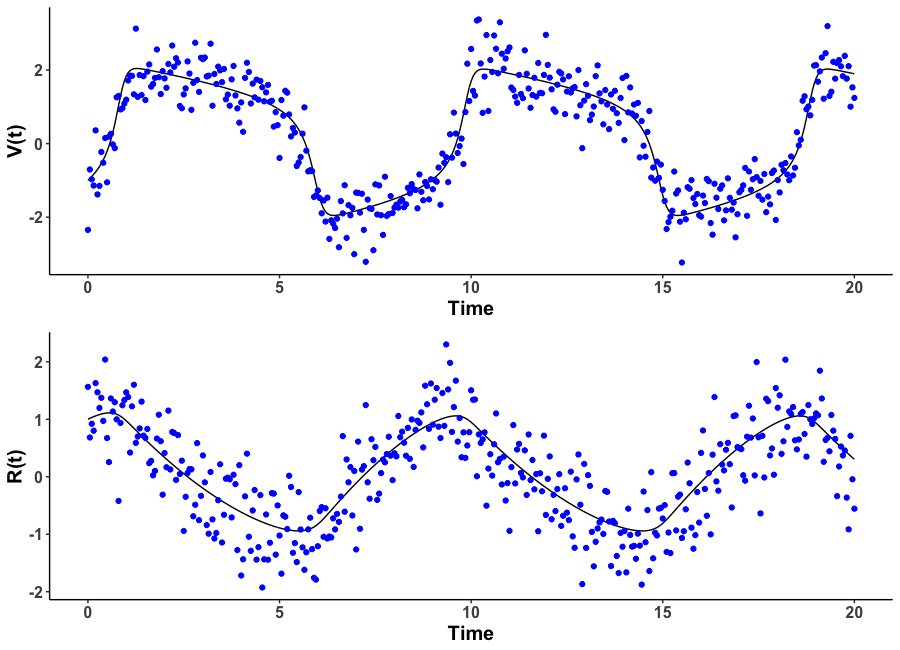
\includegraphics[width=\textwidth]{FH_observation.png}
\caption{\label{fig:FHN_2d} Given the known FitzHugh-Nagumo model, we are able to generate the true solutions. In this case, we set the parameters to be $(a,b,c) = (0.2,0.2,3)$ and are able to generate the true solution of the system, $V(t)$ and $R(t)$. The top graph demonstrates the solution $V(t)$, the black line, whereas the bottom graph shows the solution $R(t)$. For parameter estimations, we have added random noises to the true solution and use observations as the blue points in both graphs.}
\end{figure}
First step of estimating parameters is to declare basis object for each state variable. For observation period from time 0 to time 20, the basis is defined on 101 knots with B-spline basis function of order of 4. The total number of nuisance parameters is 103. For this example, the same basis will be used for both dimensions $V$ and $R$:
\begin{example*}
knots  <- seq(0, 20, length.out = 101)
norder <- 4
nbasis <- length(knots) + norder - 2
basis  <- create.bspline.basis(c(0, 20), nbasis, norder, breaks = knots)
basis.list <- list(basis, basis)
\end{example*}
Then, \code{pcode} can be executed as follows:
\begin{example*}
pcode.result <- pcode(
  data = observ[, 2:3], time = times, ode.model = Dmodel,
  par.names = c("a", "b", "c"), state.names = c("V", "R"),
  par.initial = rnorm(3), lambda = 1e2,
  basis.list = basis.list
)

pcode.result['structural.par']
0.1953324 0.2203495 2.9269980

\end{example*}



In addition, we can also compare the estimation performance of the proposed package \pkg{pCODE} with the existing package \pkg{CollocInfer}. Figure~\ref{fig:comparison} summarizes the comparison between two packages on the parameter estimation of the Fitz-Hugh Nagumo model. 

\begin{figure}[H]
  \centering 
  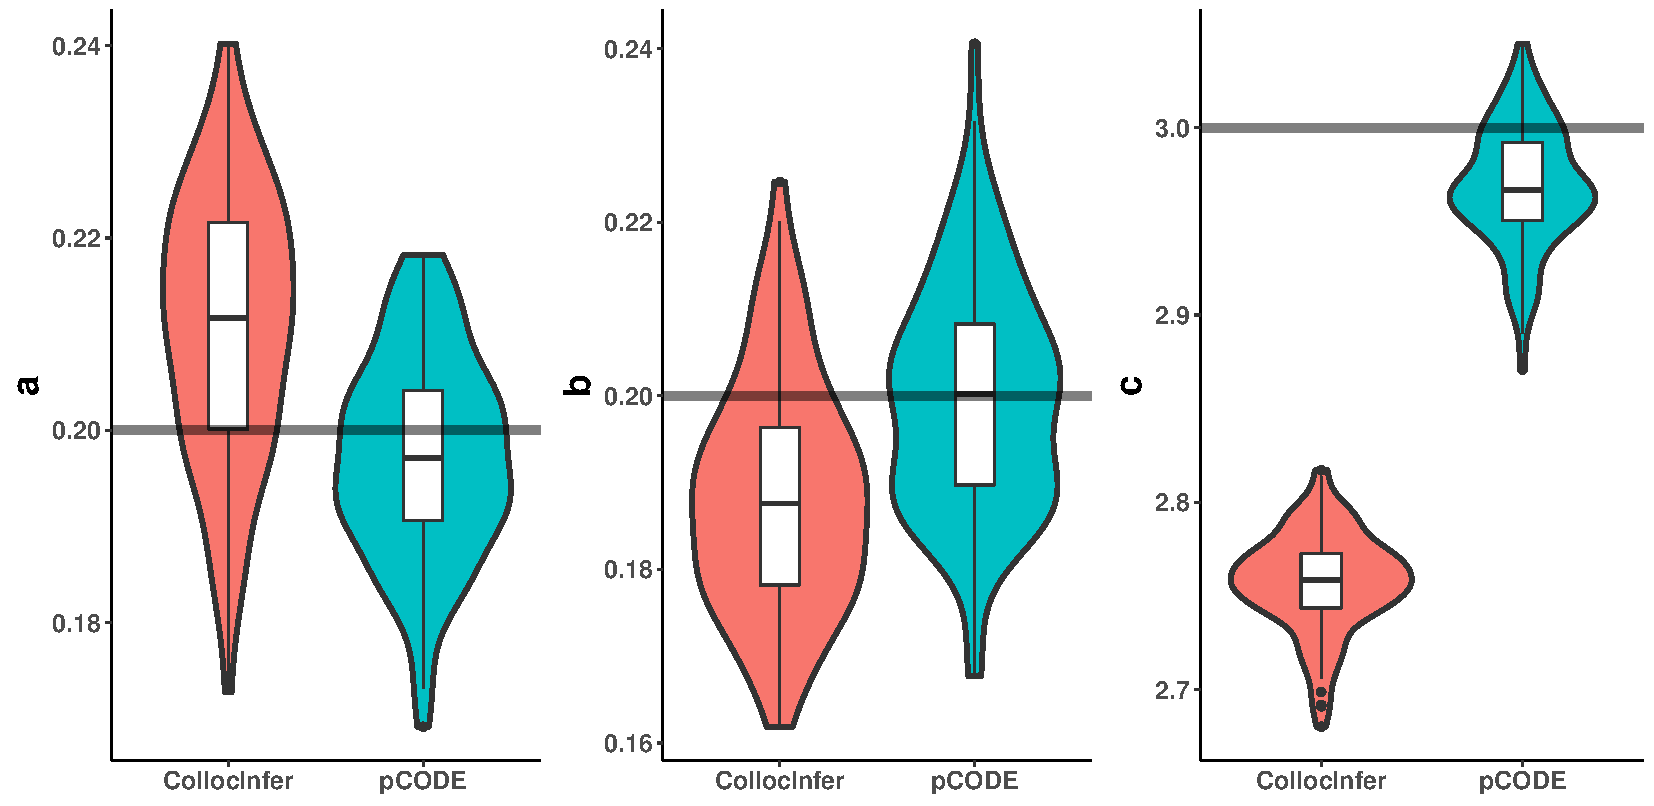
\includegraphics[width=\textwidth]{comparisonbetweentwopackages.pdf}
  \caption{\label{fig:comparison} We have repeated the data generation and parameter estimation for 100 times given the FitzHugh-Nagumo model. The parameter estimates of $(a,b,c)$ are summarized in the violin plots ordered from left to right. Within each replication, we also use the \lstinline{CollocInfer} package for parameters estimation. In each plot, the blue violion plot contains estimates from \lstinline{pCODE} whereas the red one contains those from \lstinline{CollocInfer}. The black horizontal lines correspond to the true model parameters used for simulating data sets.}
\end{figure}

Package \pkg{CollocInfer} requires the Jacobian and Hessian matrices for estimating the parameters of the ODE models, whereas the proposed \pkg{pCODE} package is a derivative-free method. Both packages are estimating parameters a and b with satisfaction, and the estimates from both methods cover the true values. However, we can see that \pkg{pCODE} produced better estimations for the third parameter c in the model. Our package does not depend on users to provide tedious details but still performs equally well in parameter estimations. 




As a part of the estimation routine, we can use two methods for estimating the variance of structural parameters. First, the usage of bootstrap variance estimator is 
\begin{example*}
bootsvar.res <- bootsvar(
  data = data, time = observ[, 1], ode.model = ode.model,
  par.names = c("a", "b", "c"), state.names = c("V", "R"),
  par.initial = c(0.15, 0.25, 5), lambda = 1e2, basis.list = basis.list,
  controls = list(smooth.lambda = 10, verbal = 1, maxeval = 20), bootsrep = 20
)

\end{example*}
based on a bootstrap sample with size of 20. Delta variance estimator is much faster in approximating the variance through the following execution
\begin{example*}
deltavar.res <- deltavar(
  data = observ[, 2:3], time = observ[, 1], ode.model = Dmodel,
  par.names = c("a", "b", "c"), state.names = c("V", "R"), par.initial = c(0.1, 0.3, 4),
  lambda = 1e2, basis.list = basis.list,
  stepsize = 0.001, y_stepsize = 0.001
)
\end{example*}



\subsection{Non-normal errors}
The previous examples assume that the random errors are following Normal distributions, hence the optimization utilizes the routines of NLS problems. In some cases, if the state variables are bounded or the errors have a non-normal distribution, a likelihood (or log-likelihood) function can be passed to the function \code{pcode} in order to evaluate the objective functions. Subsequently, the function \code{pcode} will be using \code{optim} for optimizations of both inner and outter objective functions. \par 
The first example would reuse the simple ODE model, i.e., 
\begin{equation*}
\dot{X} = \theta X (1-\frac{X}{10}).
\end{equation*}
In this case, the observations are simulated where log-normal errors are added to the solution of the ODE model in the following way:
\begin{equation*}
log(y_{i}) = log(x_{i}) + \epsilon_{i}
\end{equation*}
where $\epsilon_{i} \sim N(0,\sigma^{2})$. One simulated data is illustrated in the following Figure~\ref{fig:lognormal}:
\begin{figure}[H]
\centering 
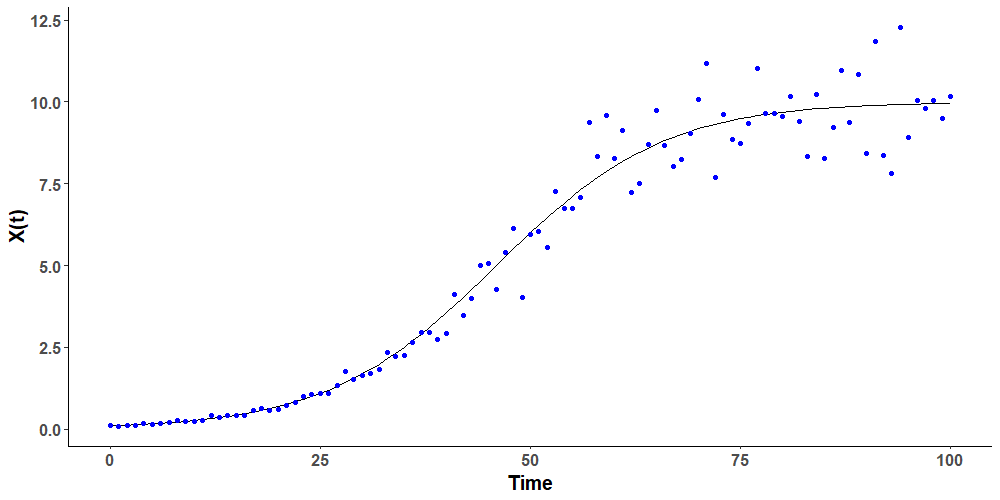
\includegraphics[width=\textwidth]{log_observation.png}
\caption{\label{fig:lognormal} This plots illustrates that observations from ODE systems can follow a non-normal distribution. Given the previous simple ODE model, we generate random noises from a log-normal distribution and add them to the true solution of the system. Black line represents the solution of the simple ODE system, and simulated observations are indicated by blue points.}
\end{figure}
While keeping all the original settings for \code{pcode}, a log-likelihood function, as $g(\bm{e}_{i}|\cdot)$ in both~\ref{eq:innerobj} and~\ref{eq:outterobj}, is additionally specified as follows
\begin{example*}
likfun <- function(x) \{
  res <- lapply(x, function(t) {
    dnorm(t,
      mean = 0,
      sd = 0.1, log = TRUE
    )
  })
  return(sum(unlist(res)))
\}
\end{example*}
Instead of defining the likelihood only as a function of residuals, \code{pcode} allows full flexibility in constructing a likelihood as long as it returns the evaluation. Then, the likelihood function can be passed to \code{pcode} through the argument \code{likelihood.fun} with specification of a basis object for interpolation
\begin{example*}
knots <- seq(0, 100, length.out = 21)
norder <- 4
nbasis <- length(knots) + norder - 2
basis <- create.bspline.basis(c(0, 100), nbasis, norder, breaks = knots)
lkh.result <- pcode(
  data = observ, time = times, likelihood.fun = likfun,
  par.initial = 0.1, ode.model = ode.model,
  basis.list = basis, par.names = "theta", state.names = "X", lambda = 1e2
)
lkh.result["structural.par"]
0.105                  
\end{example*}
\section{Summary} \label{sec:summary}
In this article, we have reviewed the parameter cascade method for estimating ordinary differential equations and introduced the new package \pkg{pCODE} for implementing this method. \pkg{pCODE} offers a derivative-free procedure to estimate any ODE models where its functions are easily understood and to apply.  Several examples of ODE models are considered for assessing the performance of functions from \pkg{pCODE} involving estimating parameters, producing variability measures, and tuning hyper-parameters. Subsequently, we can observe that the implemented functions provide satisfactory results presented with details in the fourth section. Type of examples differs in both model complexity and error distribution. Furthermore, a special case of predator-prey model is studied when some state variables are completely missing from observations. The package is able to simplifies the application procedure and reproduce the estimation results as in \cite{Jiguo}. 

One of the future works is to expand the flexibility of this package. Even though \pkg{pCODE} can provide satisfactory parameter estimates, current functions do not allow users to input the Jacobian and Hessian matrices to speed up the optimization process. In future package developments, we will implement the functionality to allow the input of these matrices. One limitation of the package is the time performance of procedures, especially for the calculation of the bootstrap variance estimator. For that matter, we are implementing this function with parallel computation ability to speed up the calculation. Moreover, we plan to expand the functionalities of the package to include data visualizations and generations of diagnostic plots and summaries.


\bibliography{pcode_rjournal}

\address{Haixu Wang\\
  Simon Fraser University\\
  8888 University Dr, Burnaby, BC V5A 1S6 \\
  Canada\\
  \email{haixuw@sfu.ca}}

\address{Jiguo Cao\\
Simon Fraser University\\
8888 University Dr, Burnaby, BC V5A 1S6 \\
Canada\\
  \email{jiguoc@sfu.ca}}



